\documentclass[runningheads]{llncs}
\usepackage[hyphens]{url}
\usepackage{graphicx}
\usepackage{amsmath}


\begin{document}

\title{Genetic Model Design for 2021 Huawei Delivery Optimization Competition}

\author{Zhenshuo Chen\inst{1}\orcidID{0000-0003-2091-4160} \and
    Guowen Liu\inst{2}\orcidID{0000-0002-8375-5729}}

\institute{Dublin City University, Dublin, Ireland \and
    Trinity College Dublin, Dublin, Ireland}

\maketitle


\begin{abstract}
We design a genetic model for 2021 Huawei Delivery Optimization Competition,
which aims to minimize multi-vehicle transportation costs within the constraints of vehicle specifications.
We use the one-dimensional array as genotype to represent the transportation routes of multiple vehicles.
This representation allows us to directly use existing genetic algorithms for multi-vehicle route optimization.

\keywords{Genetic Algorithm \and Multi-vehicle Route Optimization.}
\end{abstract}


\section{INTRODUCTION}
The competition task is to takes care of deliveries of consumables from a depot to customers, as shown in Fig.~\ref{fig:overview}.

\begin{figure}[htbp]
    \centerline{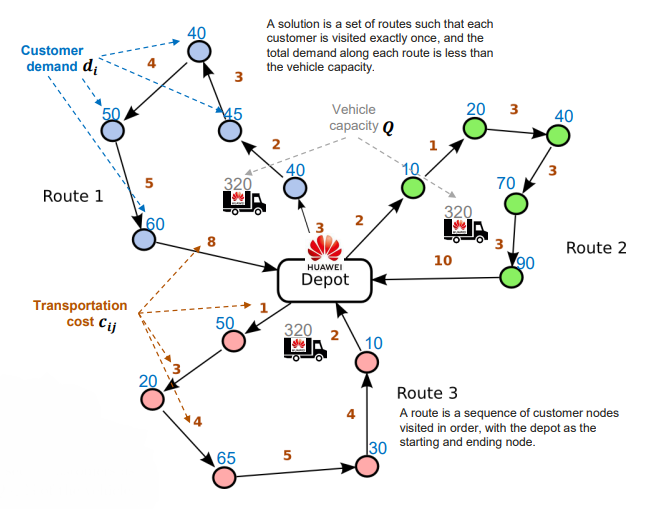
\includegraphics[width=0.8\linewidth]{figures/overview.png}}
    \caption{The overview}
    \label{fig:overview}
\end{figure}

\begin{itemize}
    \item
    The depot has a given set of home vehicles, each with a certain capacity for carrying consumables.

    \item
    Customers are represented as nodes in a graph, in which edges have an associated transportation cost equal to the distance between the nodes.

    \item
    Each customer node has an associated demand for a consumable.
\end{itemize}

The target is to minimize the total transportation cost by determining a set of routes that meet the following requirements:

\begin{itemize}
    \item Each vehicle has one route that starts and finishes at the depot.

    \item Each customer is visited exactly once.

    \item The total demand along each route is less than the vehicle capacity.
\end{itemize}

In a route, the depot is represented by node $1$ and customer numbers start from node $2$.
For example, the route $[1, 2, 3, 4, 1]$ means a vehicle starts from the depot ($1$), visits customer nodes $2$, $3$, $4$ and returns to the depot ($1$).


\section{MODEL DESIGN}
We used the genetic algorithm as our main process.
It simulates the process of natural selection which means those species who can adapt to changes in their environment are able to survive, reproduce and go to next generation as Fig.~\ref{fig:genetic}.

\begin{figure}[htbp]
    \centerline{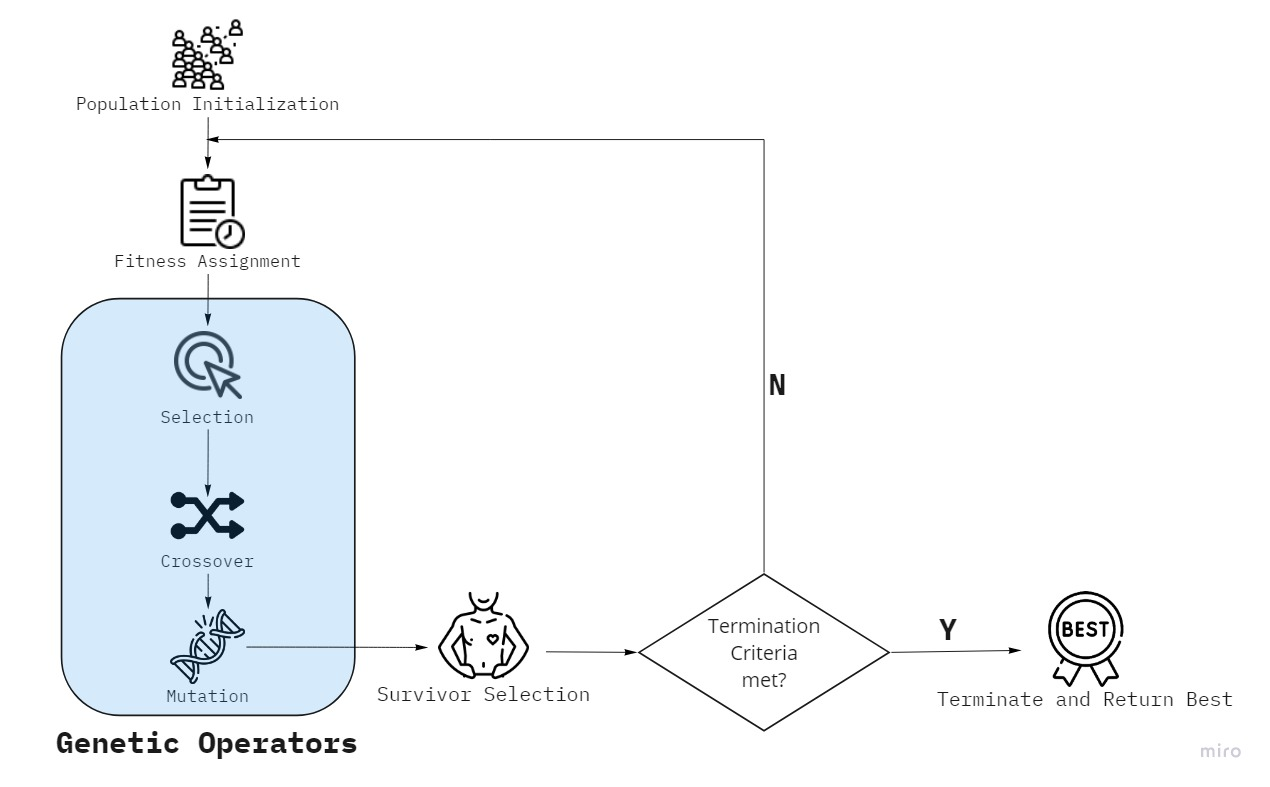
\includegraphics[width=\linewidth]{figures/genetic.jpg}}
    \caption{A genetic model}
    \label{fig:genetic}
\end{figure}

\subsection{Individual}
For a task containing $N$ customers and $M$ vehicles, we used a permutation of $N + M - 1$ consecutive numbers (0-based) to represent a transportation plan, consisting of both customers and depots.
$M - 1$ depots can split the customers into $M$ segments. Each segment represents a route.
For instance, if a task contains eight customers and three vehicles, a transportation plan can be generated as Fig.~\ref{fig:individual}.
In the example individual, $0, \ldots, 7$ are customers and $8, 9$ are the depot.

\begin{figure}[htbp]
    \centerline{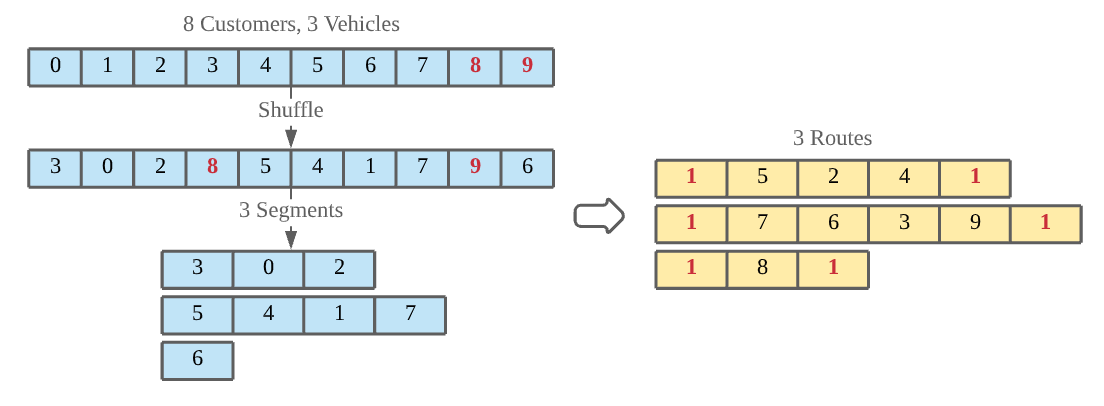
\includegraphics[width=\linewidth]{figures/individual.png}}
    \caption{Using an individual to represent multi-vehicle routes}
    \label{fig:individual}
\end{figure}

This representation can produce empty routes such as the individual $[3,0,1,2]$ for a task containing three customers and two vehicles.
The depot $3$ is in the first position, so the routes are $[1, 1]$ and $[1, 2, 3, 4, 1]$, transformed from an empty segment and $[0,1,2]$.

\subsection{Mutation}
In a mutation operation, we randomly swapped the order of two nodes as Fig.~\ref{fig:mutation}.

\begin{figure}[htbp]
    \centerline{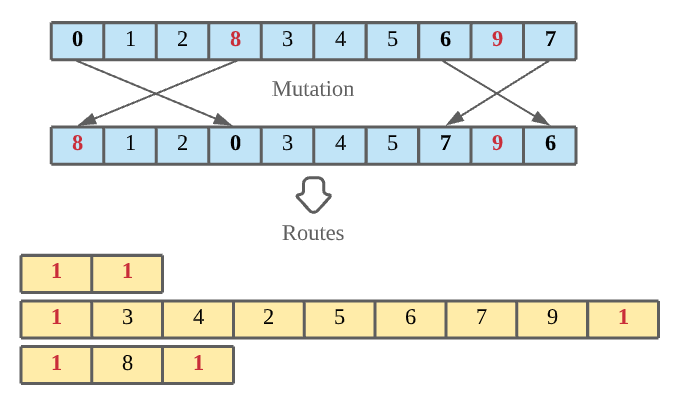
\includegraphics[width=0.8\linewidth]{figures/mutation.png}}
    \caption{Mutation}
    \label{fig:mutation}
\end{figure}

\subsection{Crossover}
In a crossover operation, we executed ordered crossover on two parents to produce children, as shown in Fig.~\ref{fig:crossover}.

\begin{figure}[htbp]
    \centerline{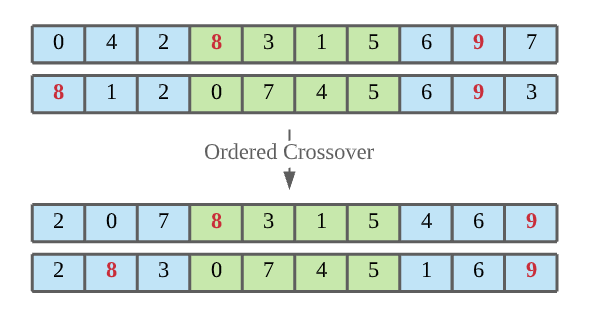
\includegraphics[width=0.8\linewidth]{figures/crossover.png}}
    \caption{Ordered crossover}
    \label{fig:crossover}
\end{figure}

\subsection{Selection}
We use tournament selection, keeping transportation plans with the highest fitness from randomly chosen candidates.

The fitness is the cost of a transportation plan.
For overloaded plans, a large value is added to fitness as a penalty. This value increases as overload weight increases, see Equation.~\ref{eq:penalty}.

\begin{equation}
    Penalty = \sum_{i}\sum_{j}c_{i, j} + 2 \cdot W
    \label{eq:penalty}
\end{equation}

$c_{i, j}$ is the cost between the node $i$ and $j$, and $W$ is overloaded weight of the transportation plan.


\section{IMPLEMENTATION}
Our implementation is based on \verb|DEAP| framework \cite{deap}.
The source code is available on the GitHub \footnote{\url{https://github.com/Zhuagenborn/Huawei-Delivery-Optimization}}.


\bibliographystyle{splncs04}
\bibliography{huawei-delivery-optimization}

\end{document}